\documentclass[12pt]{article}

\usepackage{amsmath, amsthm, amssymb, amsfonts}
\usepackage{derivative, cancel, hyperref, bookmark}
\usepackage[english]{babel}
\usepackage[Rejne]{fncychap}
\usepackage[utf8]{inputenc}
\usepackage[T1]{fontenc}
\usepackage{mathpazo}
\usepackage{caption, subcaption}
\usepackage[dvipsnames]{xcolor}
\usepackage{tcolorbox, color, soul}
\usepackage[a4paper, portrait, margin=1.5cm]{geometry}
\tcbuselibrary{theorems, skins, breakable}
\hypersetup{colorlinks=true, linkcolor=blue, filecolor=magenta, urlcolor=cyan}
\usepackage{float}
\usepackage{xcolor}
\usepackage{graphicx}
\usepackage{media9} % Package to include videos


\begin{document}

\begin{titlepage}
    \newcommand{\HRule}{\rule{\linewidth}{0.5mm}}
    \center

    % Headings
    \textsc{\Huge Systems and Control Engineering}\\[1.5cm]
    \textsc{\LARGE\bfseries SC649: Embedded Controls and Robotics}\\[1cm] % Major heading

    % Title
    \HRule\\[0.4cm]
    {\huge\bfseries Assignment 3}\\[0.2cm] % Title of your document
    \HRule\\[1.5cm]

    % Author(s)
    \begin{minipage}{0.4\textwidth}
        \begin{flushleft}
            \large
            \textit{Team}\\
            \textsc{Pranav Gupta} (\texttt{22B2179})\\
            \textsc{Rohan Mekala} (\texttt{22B2106})\\
            \textsc{Sahil Sudhakar} (\texttt{210010055})\\
        \end{flushleft}
    \end{minipage}
    ~
    \begin{minipage}{0.4\textwidth}
        \begin{flushright}
            \large
            \textit{Instructor}\\
            \textsc{Prof. Leena Vachhani}\\
            % \href{mailto:leena.vachhani@iitb.ac.in}{leena.vachhani@iitb.ac.in}
        \end{flushright}
    \end{minipage}

    % Logo
    \vfill\vfill\vfill
    \includegraphics[width=0.4\textwidth]{/home/pranav/Documents/LaTeX/SysCon/logo.png}\\[1cm]

    % Date
    \vfill\vfill
    {\LARGE \today}
    \vfill

\end{titlepage}

\pagebreak
\tableofcontents

\section*{Work Distribution}
\begin{enumerate}
	\item \textbf{Pranav Gupta} (\texttt{22B2179}): understanding frenet frame and python implementation
	\item \textbf{Rohan Mekala} (\texttt{22B2106}): understanding the model and control law
	\item \textbf{Sahil Sudhakar} (\texttt{210010055}): automation of running test cases and data visualisation
\end{enumerate}

\pagebreak

\section{Choice of Amplitude for Reference Trajectory}

\subsection{Observations}
For different amplitudes:
\begin{itemize}
    \item \textbf{$A = 5$}:
          % \begin{itemize}
          %     \item A smaller trajectory radius results in tighter curves.
          %     \item The robot tracks the trajectory closely, with minor deviations due to the relatively easy path.
          \begin{figure}[H]
              \centering
              \includemedia[
                  width=0.8\linewidth,
                  height=0.45\linewidth,
                  activate=onclick,
                  addresource=Figs/A_5_k1_4_k2_4.mp4,
                  flashvars={
                          source=Figs/A_5_k1_4_k2_4.mp4
                          &loop=true  % Loops the video
                          &autoplay=true  % Autoplay the video
                      }
              ]{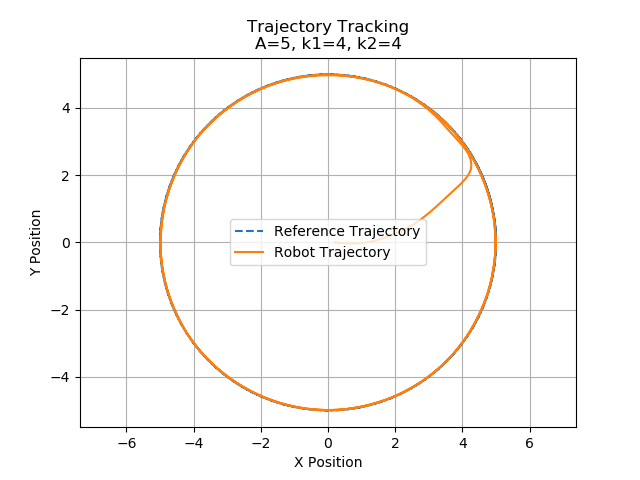
\includegraphics[width=0.8\linewidth]{Figs/A_5_k1_4_k2_4_trajectory.png}}{VPlayer.swf}
              \caption{Trajectory Tracking for $A = 5$ (Click to play)}
          \end{figure}
          % \end{itemize}
    \item \textbf{$A = 8$}:
          % \begin{itemize}
          %     \item A moderate amplitude allows the robot to follow the trajectory with more visible corrections.
          %     \item Tracking errors are noticeable but manageable, indicating a balanced control difficulty.
          \begin{figure}[H]
              \centering
              \includemedia[
                  width=0.8\linewidth,
                  height=0.45\linewidth,
                  activate=onclick,
                  addresource=Figs/A_8_k1_4_k2_4.mp4,
                  flashvars={
                          source=Figs/A_8_k1_4_k2_4.mp4
                          &loop=true
                          &autoplay=true
                      }
              ]{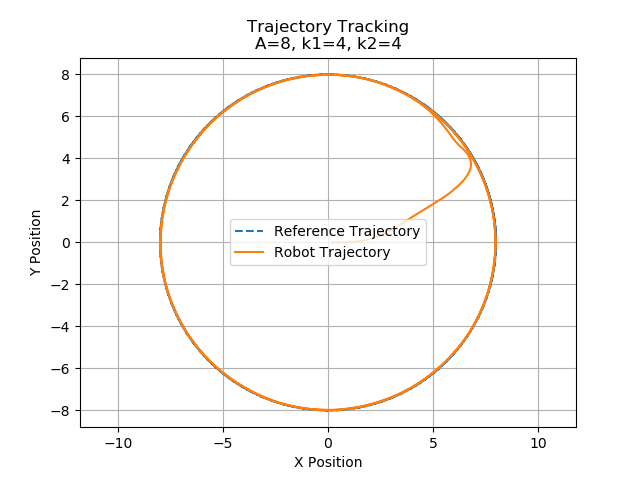
\includegraphics[width=0.8\linewidth]{Figs/A_8_k1_4_k2_4_trajectory.png}}{VPlayer.swf}
              \caption{Trajectory Tracking for $A = 8$ (Click to play)}
          \end{figure}
          % \end{itemize}
    \item \textbf{$A = 12$}:
          % \begin{itemize}
          %     \item A larger amplitude increases the curve radii, leading to more challenging tracking.
          %     \item Deviations become more pronounced as the robot struggles to maintain the trajectory, especially at higher $\omega$ values.
          \begin{figure}[H]
              \centering
              \includemedia[
                  width=0.8\linewidth,
                  height=0.45\linewidth,
                  activate=onclick,
                  addresource=Figs/A_12_k1_4_k2_4.mp4,
                  flashvars={
                          source=Figs/A_12_k1_4_k2_4.mp4
                          &loop=true
                          &autoplay=true
                      }
              ]{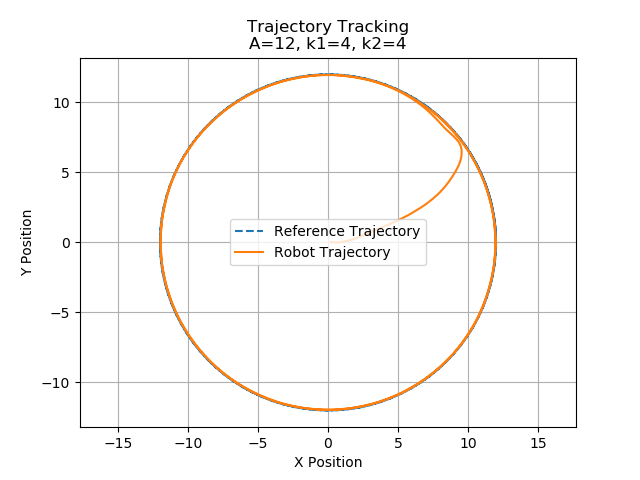
\includegraphics[width=0.8\linewidth]{Figs/A_12_k1_4_k2_4_trajectory.png}}{VPlayer.swf}
              \caption{Trajectory Tracking for $A = 12$ (Click to play)}
          \end{figure}
          % \end{itemize}
\end{itemize}

\noindent link: \url{drive.google.com/drive/folders/1gWPNkXLT5S5GkosSYY6G4AvSyILF0KUd?usp=sharing} to folder containing experimental results (\texttt{.csv}, \texttt{.png}, \texttt{.gif}, \texttt{.mp4})

\subsection{Analysis}

The controller is generally successful in tracking the desired trajectory relatively closely, its performance naturally varying with the proportional gains. We ran a tootal of 75 runs covering all combinations of \(A\in\{5,8,12\}\) and \(k_1,k_2\in\{1,2,4,8,16\}\). From these, we draw the following insights:

\begin{enumerate}
    \item Increasing \(A\) primarily increases the settling time, with the transient and steady state responses scaling accordingly to maintain their characteristics.
    \item Transient response is smoother for cases where \(k_1\sim k_2\) and squigglier otherwise.
\end{enumerate}

\noindent\textbf{Steady State}
\begin{enumerate}
    \item The steady state trajectory of the controller when \(k_1=k_2\) is approximately uniform circular motion.
    \item Whenever \(k_2>k_1\), the emergent steady state trajectory is distended along the 1st and 3rd quadrants, the eccentricity increasing with \(k_2/k_1\).
    \item Similarly, \(k_1>k_2\) results in steady state trajectories distended along the 2nd and 4th quadrants, the eccentricity increasing with \(k_1/k_2\).
    \item In cases of slight imbalance, the steady state trajectory remains within the desired circle. However in cases of high imbalance, the steady state trajectory may even overshoot the reference trajectory. 
\end{enumerate}


\section{Effect of Control Gains $(K_1, K_2)$ on Tracking Performance}


\subsection{Observations}
\begin{figure}[H]
    \centering
    \captionsetup{justification=centering}

    % First row of the grid
    \subfloat[$K_1=1, K_2=1$]{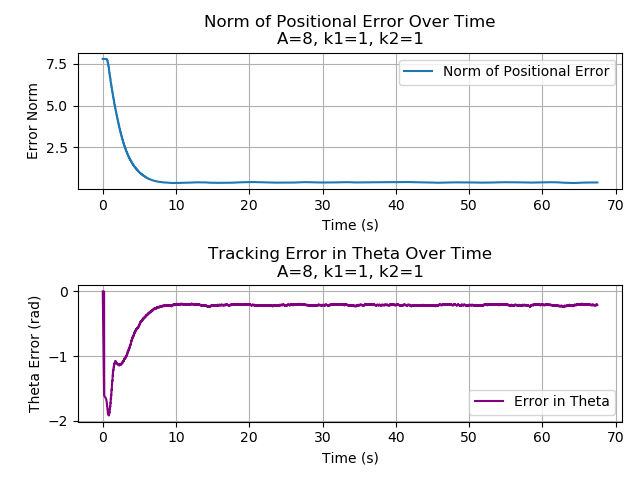
\includegraphics[width=0.19\linewidth]{Figs/A_8_k1_1_k2_1_errors.png}} \hfill
    \subfloat[$K_1=1, K_2=2$]{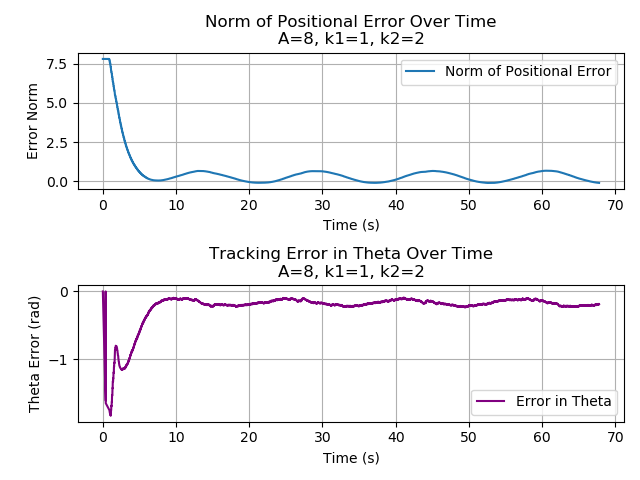
\includegraphics[width=0.19\linewidth]{Figs/A_8_k1_1_k2_2_errors.png}} \hfill
    \subfloat[$K_1=1, K_2=4$]{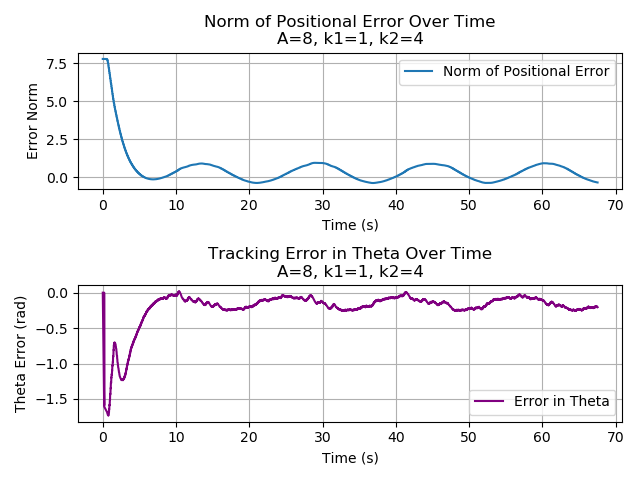
\includegraphics[width=0.19\linewidth]{Figs/A_8_k1_1_k2_4_errors.png}} \hfill
    \subfloat[$K_1=1, K_2=8$]{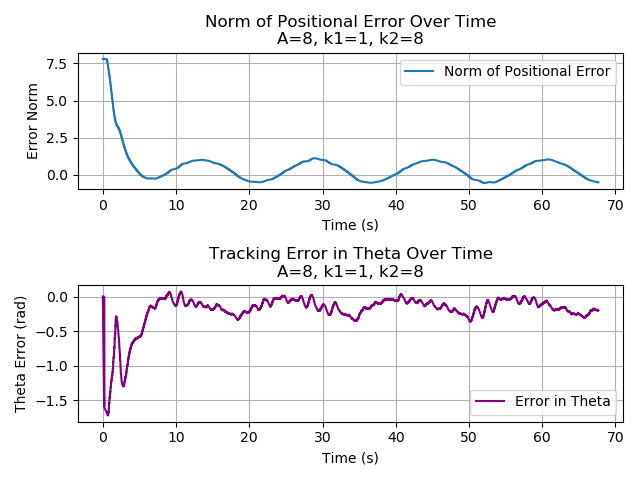
\includegraphics[width=0.19\linewidth]{Figs/A_8_k1_1_k2_8_errors.png}} \hfill
    \subfloat[$K_1=1, K_2=16$]{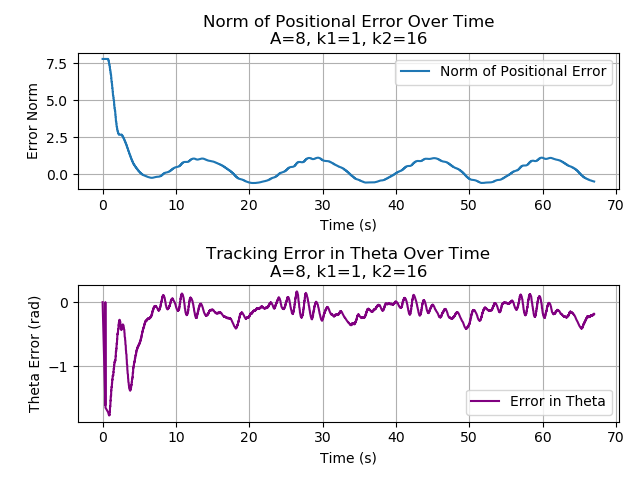
\includegraphics[width=0.19\linewidth]{Figs/A_8_k1_1_k2_16_errors.png}}

    % Second row of the grid
    \subfloat[$K_1=2, K_2=1$]{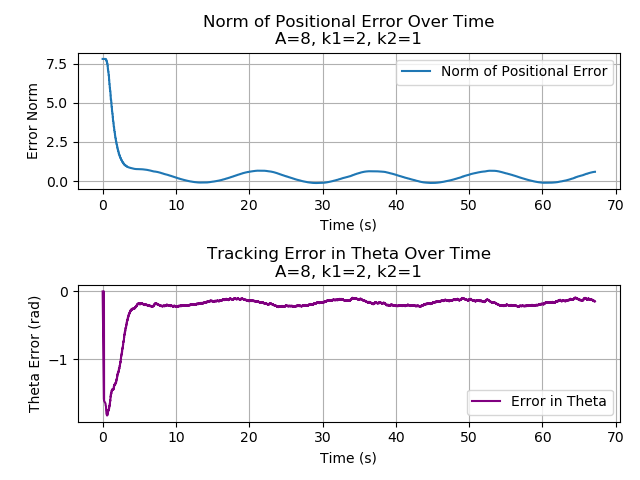
\includegraphics[width=0.19\linewidth]{Figs/A_8_k1_2_k2_1_errors.png}} \hfill
    \subfloat[$K_1=2, K_2=2$]{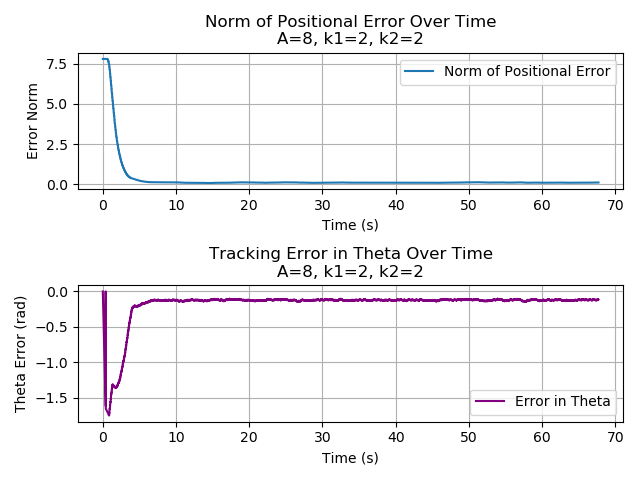
\includegraphics[width=0.19\linewidth]{Figs/A_8_k1_2_k2_2_errors.png}} \hfill
    \subfloat[$K_1=2, K_2=4$]{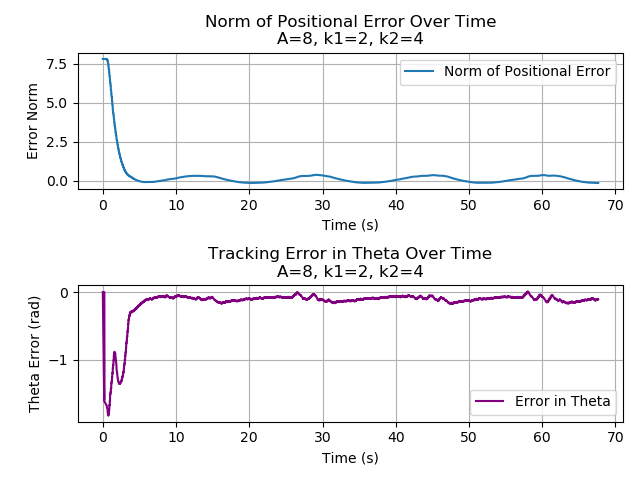
\includegraphics[width=0.19\linewidth]{Figs/A_8_k1_2_k2_4_errors.png}} \hfill
    \subfloat[$K_1=2, K_2=8$]{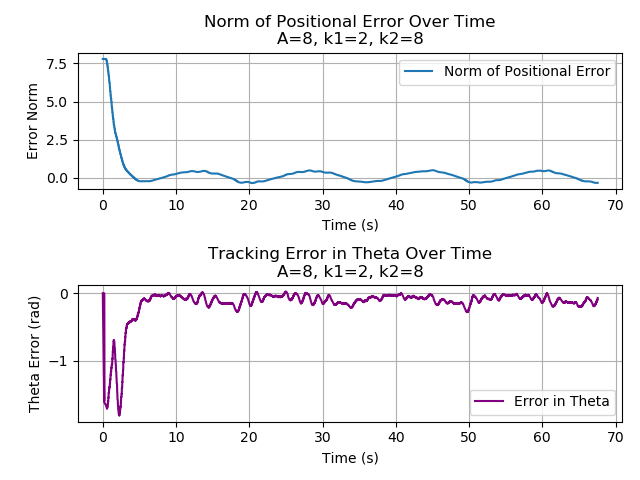
\includegraphics[width=0.19\linewidth]{Figs/A_8_k1_2_k2_8_errors.png}} \hfill
    \subfloat[$K_1=2, K_2=16$]{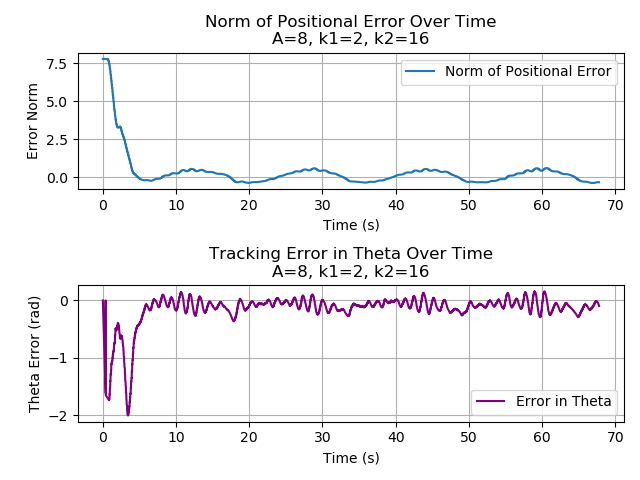
\includegraphics[width=0.19\linewidth]{Figs/A_8_k1_2_k2_16_errors.png}}

    % Third row of the grid
    \subfloat[$K_1=4, K_2=1$]{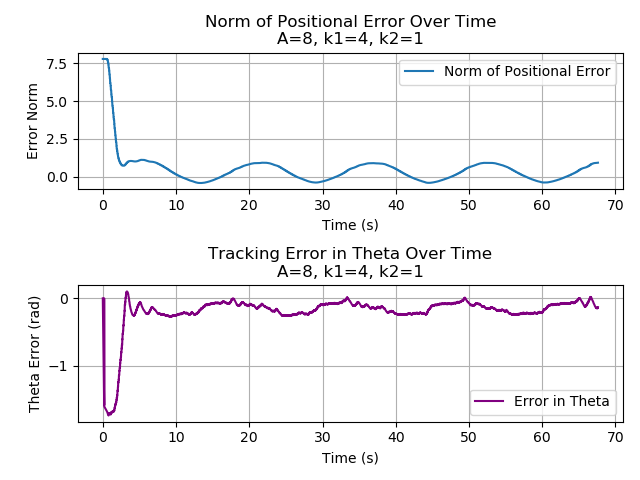
\includegraphics[width=0.19\linewidth]{Figs/A_8_k1_4_k2_1_errors.png}} \hfill
    \subfloat[$K_1=4, K_2=2$]{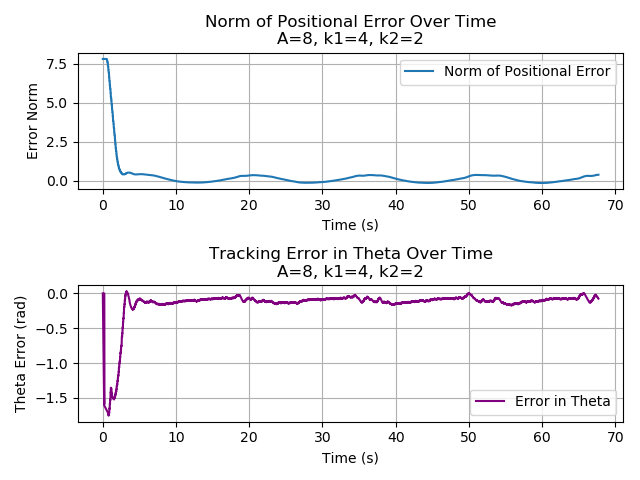
\includegraphics[width=0.19\linewidth]{Figs/A_8_k1_4_k2_2_errors.png}} \hfill
    \subfloat[$K_1=4, K_2=4$]{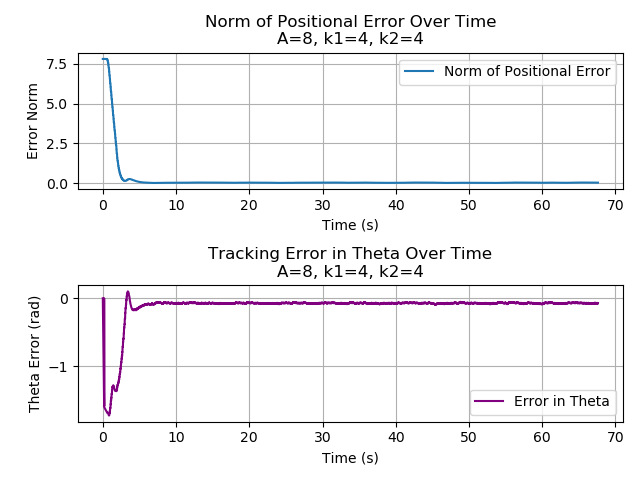
\includegraphics[width=0.19\linewidth]{Figs/A_8_k1_4_k2_4_errors.png}} \hfill
    \subfloat[$K_1=4, K_2=8$]{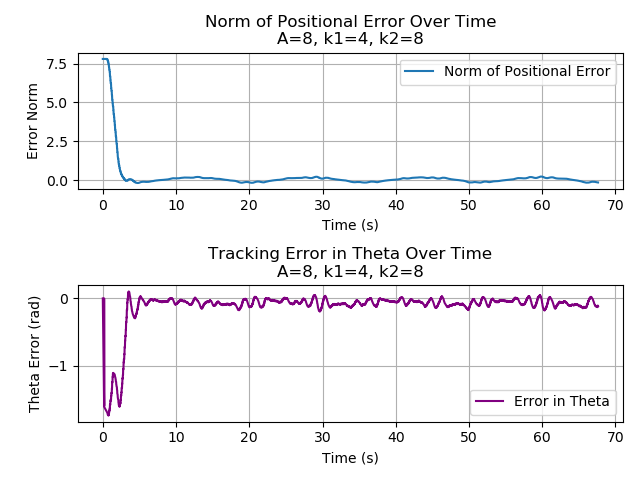
\includegraphics[width=0.19\linewidth]{Figs/A_8_k1_4_k2_8_errors.png}} \hfill
    \subfloat[$K_1=4, K_2=16$]{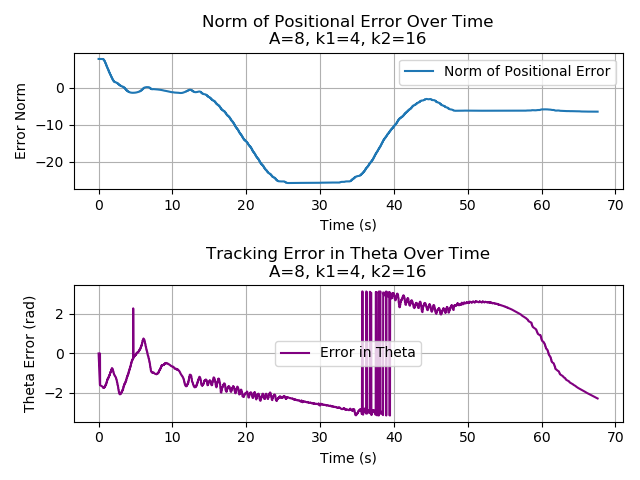
\includegraphics[width=0.19\linewidth]{Figs/A_8_k1_4_k2_16_errors.png}}

    % Fourth row of the grid
    \subfloat[$K_1=8, K_2=1$]{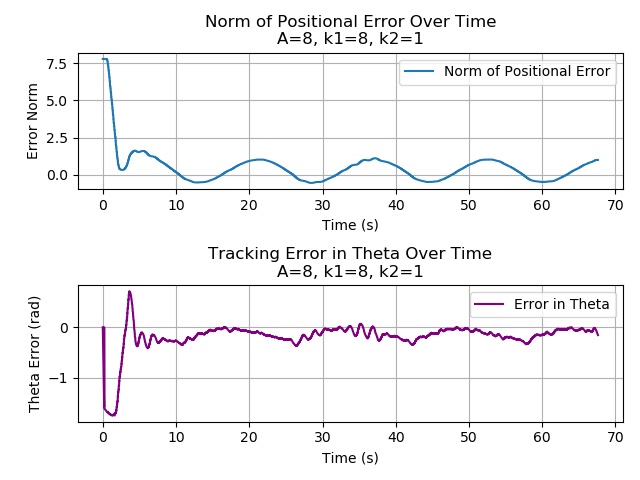
\includegraphics[width=0.19\linewidth]{Figs/A_8_k1_8_k2_1_errors.png}} \hfill
    \subfloat[$K_1=8, K_2=2$]{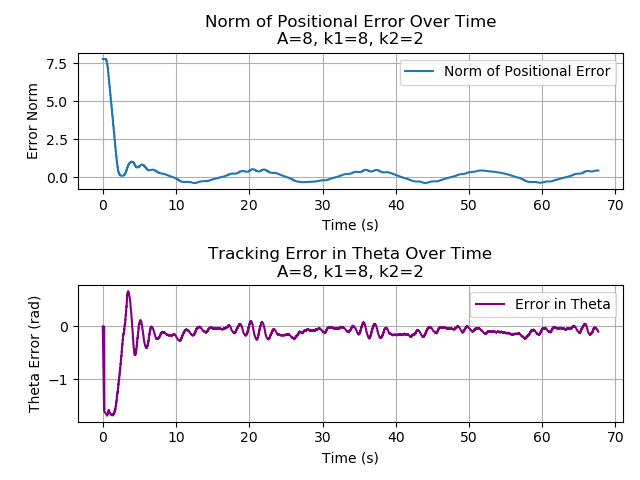
\includegraphics[width=0.19\linewidth]{Figs/A_8_k1_8_k2_2_errors.png}} \hfill
    \subfloat[$K_1=8, K_2=4$]{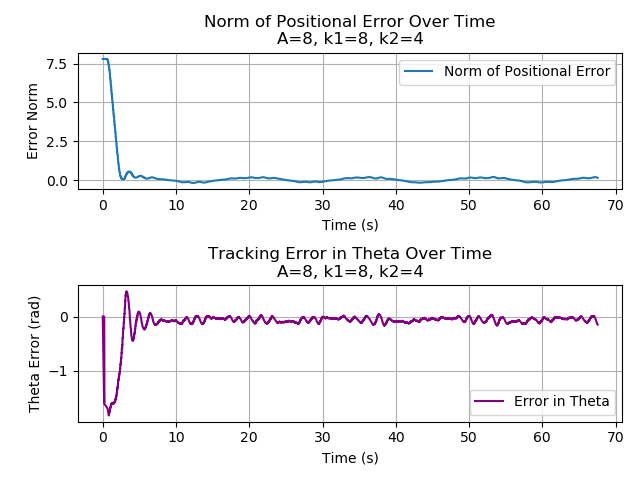
\includegraphics[width=0.19\linewidth]{Figs/A_8_k1_8_k2_4_errors.png}} \hfill
    \subfloat[$K_1=8, K_2=8$]{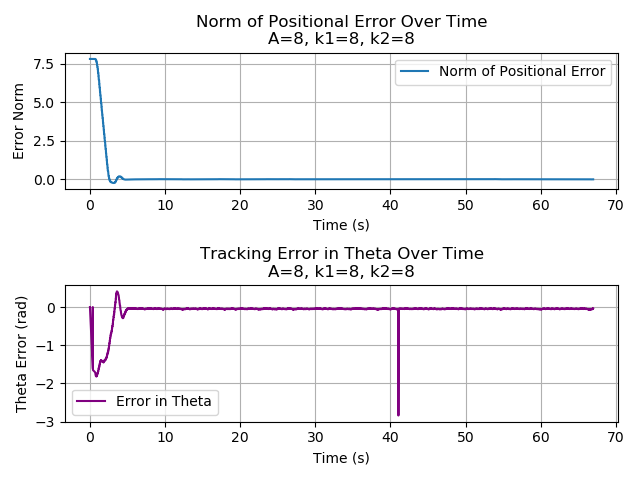
\includegraphics[width=0.19\linewidth]{Figs/A_8_k1_8_k2_8_errors.png}} \hfill
    \subfloat[$K_1=8, K_2=16$]{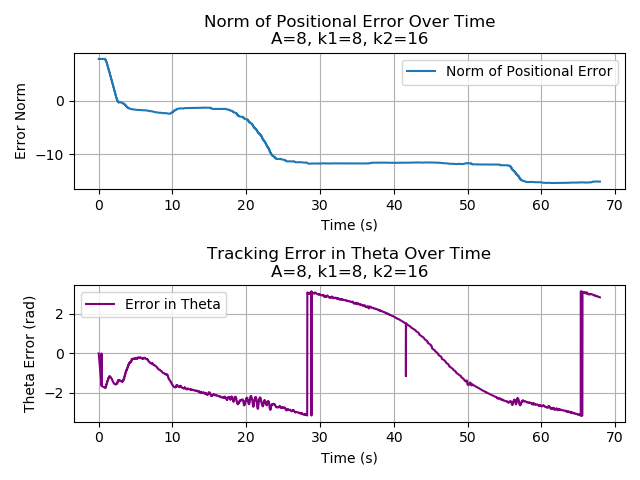
\includegraphics[width=0.19\linewidth]{Figs/A_8_k1_8_k2_16_errors.png}}

    % Fifth row of the grid
    \subfloat[$K_1=16, K_2=1$]{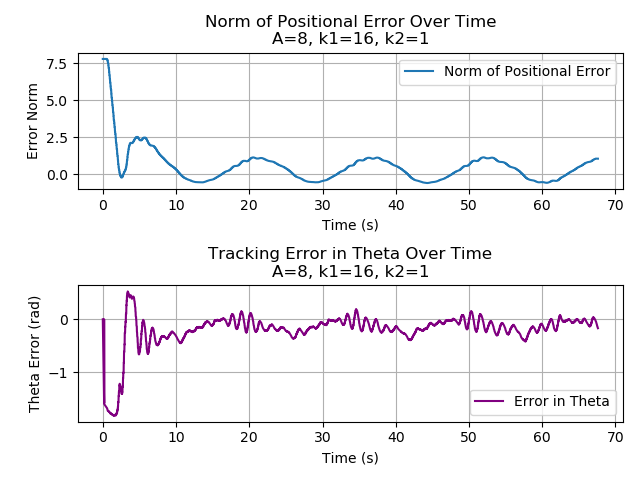
\includegraphics[width=0.19\linewidth]{Figs/A_8_k1_16_k2_1_errors.png}} \hfill
    \subfloat[$K_1=16, K_2=2$]{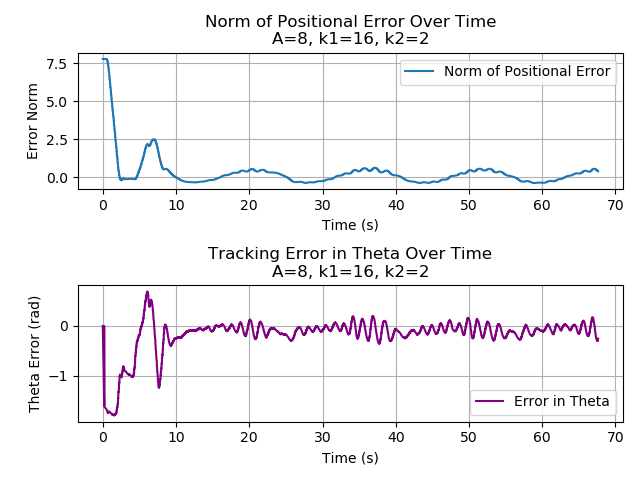
\includegraphics[width=0.19\linewidth]{Figs/A_8_k1_16_k2_2_errors.png}} \hfill
    \subfloat[$K_1=16, K_2=4$]{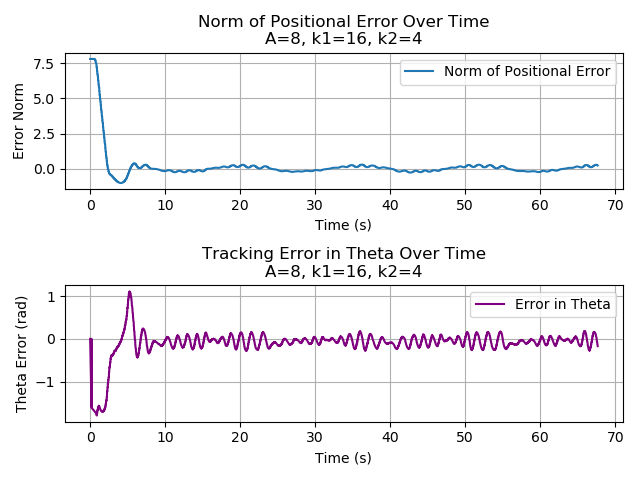
\includegraphics[width=0.19\linewidth]{Figs/A_8_k1_16_k2_4_errors.png}} \hfill
    \subfloat[$K_1=16, K_2=8$]{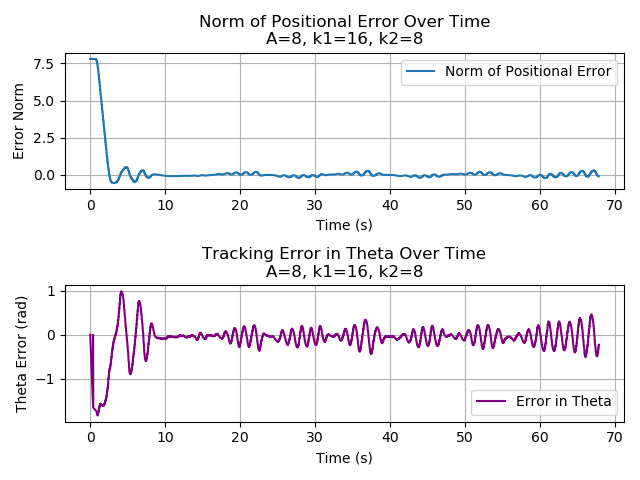
\includegraphics[width=0.19\linewidth]{Figs/A_8_k1_16_k2_8_errors.png}} \hfill
    \subfloat[$K_1=16, K_2=16$]{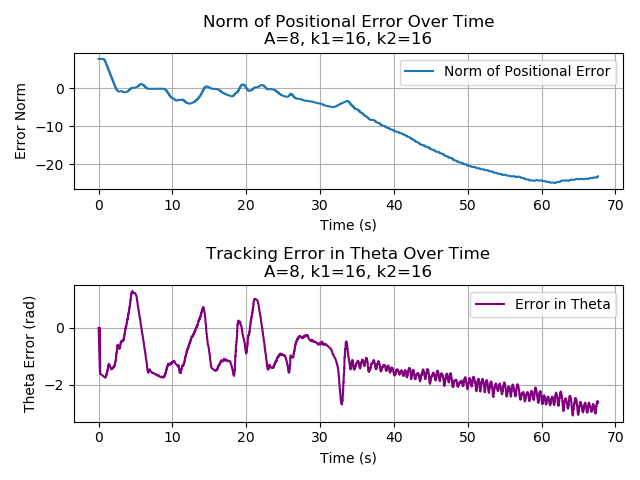
\includegraphics[width=0.19\linewidth]{Figs/A_8_k1_16_k2_16_errors.png}}

    \caption{Trajectory Tracking for Different Combinations of $K_1$ and $K_2$ (Amplitude $A=8$)}
\end{figure}

\subsection{Analysis}

As visible in the grid, a significant oscillating steady state error in the positional and angular tracking can be observed as we deviate from a \(k_1:k_2\) ratio of 1. Furthermore, higher the imbalance in the \(k_1:k_2\) ratio from 1, the more the error magnitude.\\

\textbf{1. Low Gains (\( K_1 \) and \( K_2 \) values of 1 to 4)}
\begin{itemize}
    \item \textbf{Behavior}: Slow response with visible delays in correcting errors.
    \item \textbf{Positional Error}: Gradual reduction with longer settling times, indicating under-damped behavior.
    \item \textbf{Theta Error}: Slow convergence with minimal oscillations.
\end{itemize}
\textbf{2. Moderate Gains (\( K_1 \) and \( K_2 \) values of 4 to 8)}
\begin{itemize}
    \item \textbf{Behavior}: Balanced response with quicker corrections.
    \item \textbf{Positional Error}: Faster reduction, minor oscillations indicating good stability.
    \item \textbf{Theta Error}: Effective and smooth correction.
\end{itemize}
\textbf{3. High Gains (\( K_1 \) and \( K_2 \) values of 8 to 16)}
\begin{itemize}
    \item \textbf{Behavior}: Aggressive response with over-corrections.
    \item \textbf{Positional Error}: Quick reduction with significant oscillations, indicating over-damped behavior.
    \item \textbf{Theta Error}: Rapid fluctuations with potential instability.
\end{itemize}


\section{Bijectivity of Transformation Between Control Inputs}

\begin{enumerate}
    \item \textbf{Control Inputs to Angular and Linear Velocities}:
          \[
              \begin{pmatrix}
                  v_1 \\
                  v_2
              \end{pmatrix}
              =
              \begin{pmatrix}
                  \cos\theta & -l_1 \sin\theta \\
                  \sin\theta & l_1 \cos\theta
              \end{pmatrix}
              \begin{pmatrix}
                  1 & -l_2 \\
                  0 & 1
              \end{pmatrix}
              \begin{pmatrix}
                  u_1 \\ u_2
              \end{pmatrix}
          \]
          The criteria for bijectivity of this transformation is
          \[
              \begin{vmatrix}
                  \cos\theta & -l_1 \sin\theta \\
                  \sin\theta & l_1 \cos\theta
              \end{vmatrix}
              \begin{vmatrix}
                  1 & -l_2 \\
                  0 & 1
              \end{vmatrix} \neq 0 \iff l_1 \neq 0 \iff P\text{ doesn't lie on steering wheel axle}
          \]
          which is also stated in the book in \textbf{49.3.1} \(\to\) \textit{Car}
    \item \textbf{Conversion to Steering Angle}:
          Assuming rear-wheel drive and wheelbase length $L$ of the MIT Racecar, the conversion from angular velocity $\omega$ to the steering angle $\zeta$ is given by:
          \[
              \zeta = \arctan\left(\frac{u_2 L}{u_1}\right)
          \]
          This relationship is valid only if $u_1\neq 0$. It is easy to notice that \(\zeta\) is not unique to a pair of \((u_1,u_2)\) but rather only to their ratio. Hence, this relation is clearly never bijective because it results in the same steering angle for all values of \((u_1,u_2)\) at some fixed ratio to each other.
\end{enumerate}

\end{document}